\documentclass{beamer}
%\documentclass{beamer}
\usetheme{JuanLesPins}
\usepackage{epsfig, graphics, graphicx,subfigure, amsmath}
\usepackage[spanish,es-tabla]{babel}
\decimalpoint
\usepackage{gensymb}
\usepackage[utf8]{inputenc}
\usepackage[T1]{fontenc}
\makeatletter
\newcommand\titlegraphicii[1]{\def\inserttitlegraphicii{#1}}
\titlegraphicii{}
\setbeamertemplate{title page}
{
	\vbox{}
	{\usebeamercolor[fg]{titlegraphic}\inserttitlegraphic\hfill\inserttitlegraphicii\par}
	\begin{centering}
		\begin{beamercolorbox}[sep=8pt,center]{institute}
			\usebeamerfont{institute}\insertinstitute
		\end{beamercolorbox}
		\begin{beamercolorbox}[sep=8pt,center]{title}
			\usebeamerfont{title}\inserttitle\par%
			\ifx\insertsubtitle\@empty%
			\else%
			\vskip0.25em%
			{\usebeamerfont{subtitle}\usebeamercolor[fg]{subtitle}\insertsubtitle\par}%
			\fi%     
		\end{beamercolorbox}%
		\vskip1em\par
		\begin{beamercolorbox}[sep=8pt,center]{author}
			\usebeamerfont{author}\insertauthor
		\end{beamercolorbox}
		\begin{beamercolorbox}[sep=8pt,center]{date}
			\usebeamerfont{date}\insertdate
		\end{beamercolorbox}%\vskip0.5em
		
	\end{centering}
	%\vfill
}

%
\titlegraphic{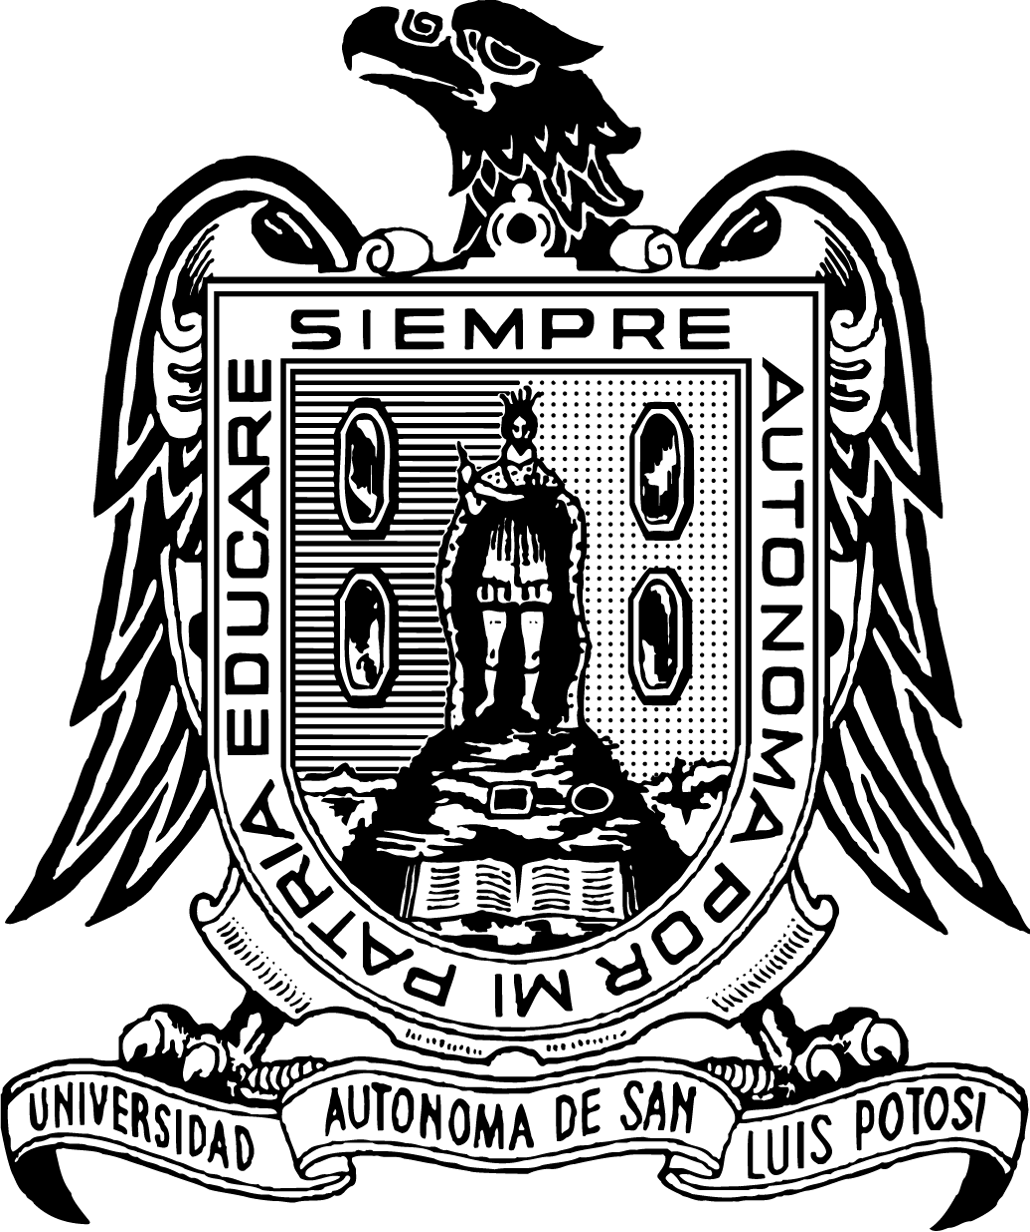
\includegraphics[scale=0.2]{portada/escudouaslp.png}}
\titlegraphicii{
\includegraphics[scale=0.15]{portada/escudofciencias.png}}
\title{Estudio te\'orico de propiedades magn\'eticas en [Pt,V] (Se,S)\textsubscript{2} y experimentación de efecto Kerr en CoFeB}
\subtitle{Cuarto avance de tesis}
\author{Gabriel adona\'i Mart\'inez Zepeda\\ \textbf{Asesor:} Dr. Ra\'ul Balderas}
\institute{Universidad Aut\'onoma de San Luis Potos\'i\\ Facultad de Ciencias}
\date{\today}


%

\usepackage[backend=bibtex,style=numeric, defernumbers=true]{biblatex}
\bibliography{refInt,refKerr,refMet,refSim,refRel}
\setbeamertemplate{bibliography item}{}
\includeonly{kerr,montaje, analisis, mediciones,concl}

\setbeamertemplate{footline}[frame number]
\begin{document}
	\frame[plain]{\titlepage}
	\frame{
		\frametitle{Contenidos}
		\tableofcontents
		\nocite{Kerr_1888,mo_2004,MOp-2008,MOp-1997,fuji_2005, Hoffmann_2019}
	}
	\section{Estudio experimental de efecto Kerr}
\subsection{Efecto Kerr magneto-\'optico}
\frame{
	\frametitle{Tipos de efecto Kerr}
    \begin{figure}[!hbt]
    	\centering
    	\subfigure[polar]{
    		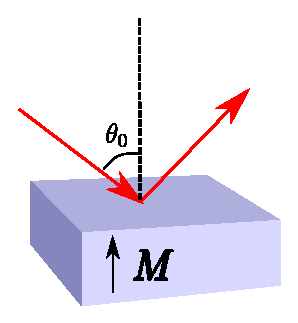
\epsfig{file=figKerr/pol/pol.eps, width=2.0cm,height=2.0cm}
    		\label{Kerr:fig:pol}
    	}
    	\subfigure[longitudinal]{
    		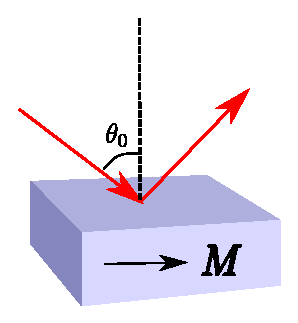
\epsfig{file=figKerr/pol/long.eps, width=2.0cm,height=2.0cm}
    		\label{Kerr:fig:long}
    	}
    	\subfigure[transversal]{
    		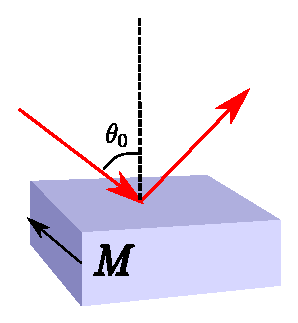
\epsfig{file=figKerr/pol/trans.eps, width=2.0cm,height=2.0cm}
    		\label{Kerr:fig:trans}
    	}
    	\caption[Configuraciones de Efecto Kerr magneto-\'optico.]{Diferentes configuraciones del efecto Kerr magneto-\'optico}
    	\label{Kerr:fig:Conf}
    \end{figure}
}
	\subsection{Montaje Experimental}
\frame{
	\frametitle{Montaje experimental}
	\begin{figure}
		\centering
		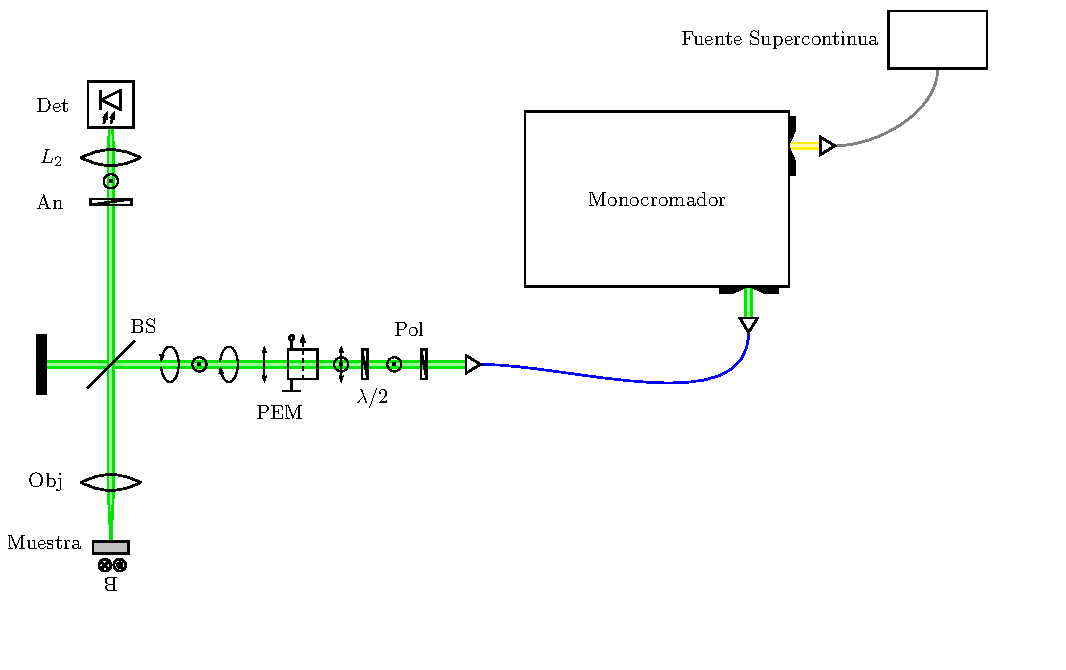
\includegraphics[scale=0.5]{figMet/diagrama/diagrama.pdf}
		\caption{Montaje Experimental}
	\end{figure}
	
}
\subsubsection{Programas de control}
\frame{
	\frametitle{Programa para adquirir la hist\'eresis}
	\begin{figure}[!hbt]
		\centering
		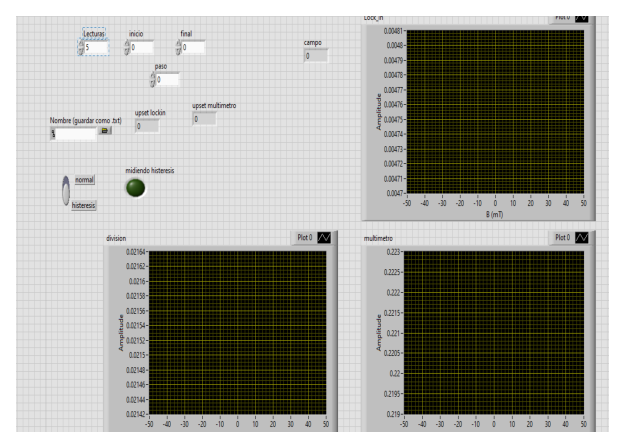
\epsfig{file=fiApLB/mk.eps, scale=0.7}
		\caption[Interfaz gr\'afica del software utilizado para obtener la hist\'eresis.]{Software para obtener la hist\'eresis. }
		\label{Lab:fig:mk}
	\end{figure}
}
\frame{
	\frametitle{Programa para adquirir espectro}
	\begin{figure}[!hbt]
		\centering
		\subfigure[Configuraci\'on]{
			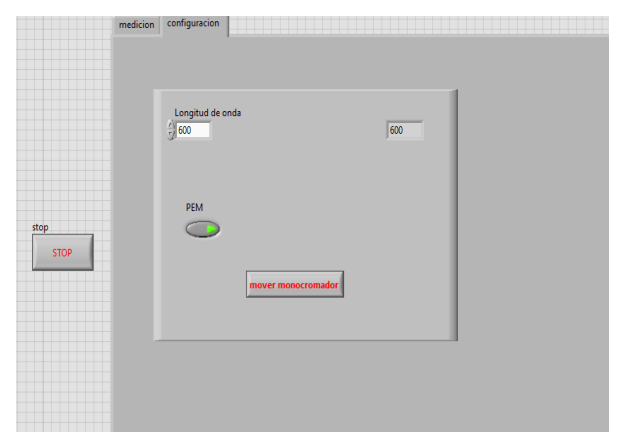
\epsfig{file=fiApLB/confEsp.eps, scale=0.4}
			\label{Lab:fig:conf}
		}
		\subfigure[Medici\'on]{
			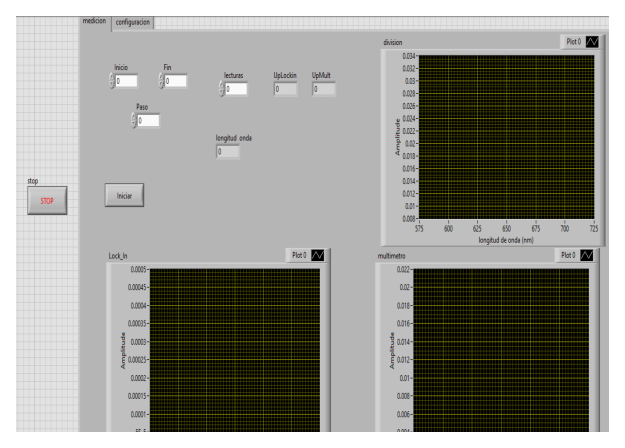
\epsfig{file=fiApLB/medEsp.eps, scale=0.4}
			\label{Lab:fig:med}
		}
		\caption[Interfaz gr\'afica del software utilizado para obtener el espectro de efecto Kerr.]{Software para obtener el espectro de efecto Kerr.}
		\label{Lab:fig:esp}
	\end{figure}
}
\endinput
	\subsection{An\'alisis del espectro}
\subsubsection{An\'alisis de Jones}
\begin{comment}


\frame{
	\frametitle{Matrices de Jones}
	\begin{itemize}
		\item Para el polarizador inicial $0 \degree $ y el analizador $90 \degree$:
		\begin{equation}
			P=
			\begin{pmatrix}
				1&0\\
				0&0
			\end{pmatrix}
			\label{Jones:ec:pol}
		\end{equation}
	\begin{equation}
		A=
		\begin{pmatrix}
			0&0\\
			0&1
		\end{pmatrix}.
		\label{Jones:ec:An}
	\end{equation}
   \pause
    \item Para el retardador de media onda para cualquier \'angulo $\theta$ :
    \begin{equation}
    	HP(\theta)= e^{\frac{-i \pi}{2}}
    	\begin{pmatrix}
    		cos(\theta)^2 - \sin(\theta)^2 & 2 \cos(\theta) \sin(\theta)\\
    		2 cos(\theta) \sin(\theta)     & \sin(\theta)^2-\cos(\theta)^2
    	\end{pmatrix},
    	\label{Jones:ec:HWP1}
    \end{equation}
    si $\theta=-22.5 \degree$:
    \begin{equation}
    	HP(-22.5\degree)= - \frac{1}{\sqrt{2}} i 
    	\begin{pmatrix}
    		1 & 1\\
    		1  & -1
    	\end{pmatrix},
    	\label{Jones:ec:HWP2}
    \end{equation}
    
	\end{itemize}
}
\frame{
	\begin{itemize}
		\item Para el modulador fotoel\'astico :
		\begin{equation}
			PEM= e^{\frac{i \pi}{4}}
			\begin{pmatrix}
				e^{i \Psi /2}&0\\
				0            &i e^{-i \Psi /2}
			\end{pmatrix}
			\label{Jones:ec:PEM},
		\end{equation}
		con 
		\begin{equation*}
			\Psi=\Psi_0 \cos(\omega t),
		\end{equation*}
		en donde $\Psi_0$ es el retardo inicial y $\omega=2 \pi f$.
	\end{itemize}
}
\frame{
	\begin{itemize}
		\item Par el divisor de haz:
		\begin{eqnarray}
			BS_r&=&
			\begin{pmatrix}
				\tilde{r}_p &0 \\
				0   &\tilde{r}_s
			\end{pmatrix} \label{Jones:ec:BSr}, \\
			BS_t&=&
			\begin{pmatrix}
				\tilde{t}_p &0 \\
				0   &\tilde{t}_s
			\end{pmatrix} \label{Jones:ec:BSt},
		\end{eqnarray}
	 con  $\tilde{r}_{p,s} = r_{p,s} e^{\delta_{p,s}}$ y $\tilde{t}_{p,s} = t_{p,s} e^{\delta_{p,s}}$.
	 \pause
	 \item Para la muestra:
	 \begin{equation}
	 	M=
	 	\begin{pmatrix}
	 		\tilde{r}_{pp}&\tilde{r}_{ps}\\
	 		\tilde{r}_{ss}&\tilde{r}_{sp}
	 	\end{pmatrix},
	 	\label{Jones:ec:Muestra}
	 \end{equation}
     con  $\tilde{r}_{pp,ss} = r_{pp,ss} e^{\delta_{pp,ss}}$ y $\tilde{r}_{pp,ss} = r_{ps,sp} e^{\delta_{ps,sp}}$ y considerando $\tilde{r}_{ps}=-\tilde{r}_{sp}$.
	\end{itemize}
	
}
\frame{
	\frametitle{Ca\'alculo de Intensidad de luz}
	\begin{equation}
		E_{sal} = A \cdot BS_t \cdot M \cdot BS_r \cdot PEM \cdot HP(-22.5 \degree) \cdot P \cdot E_{in} \label{Jones:ec:Esal} 
	\end{equation}
 \pause
 \begin{equation}
 	E_{sal} \propto A \cdot BS_t \cdot M \cdot BS_r \cdot PEM \cdot HP(-22.5 \degree) \cdot P \cdot 
 	\begin{pmatrix}
 		1\\1
 	\end{pmatrix}, \label{Jones:ec:Esal1} 
 \end{equation}
\pause
\begin{equation}
	I_{sal}= E_sal^{* T} \cdot E_sal. \label{Jones:ec:intens}
\end{equation}

}
\frame{
	Introduciendo las respectivas matrices (Ecs. \ref{Jones:ec:pol} - \ref{Jones:ec:Muestra} ) a la ecuaci\'on \ref{Jones:ec:intens}:
	\begin{equation}
		I_{sal} = \frac{t_s ^2}{2}\left( r_s^2 r_{ss}^2 + r_p^2 r_{sp}^2 \right) -r_p r_s r_{ss} r_{sp} t_{s}^2  \cos(\Psi -\delta^{(s)}+\Delta) \label{Jones:ec:Int}
	\end{equation}
    \pause
    con $\delta^{(s)}=\delta_{ss}-\delta{sp}$ y $\Delta = \delta_p - \delta_s$
    
}
\frame{
	utilizando:
	\begin{eqnarray}
		\cos(a-b)&=&\cos(a)\cos(b)+ \sin(b)\sin(a) \nonumber \\
		\sin(a+b)&=& \sin(a)\cos(b)+\cos(a)\sin(b) \nonumber 
	\end{eqnarray}
\pause
y
	\begin{eqnarray}
		\sin(\Psi_0 \cos(\omega t))&=& 2 \sum_{n=0} J_{2n+1}(\Psi_0) \cos(n \omega t) \nonumber \\
		\cos(\Psi_0 \sin(\omega t)) &=& J_0 (\Psi_0) - 2 \sum_{n=1} J_{2n} (\Psi_0) \cos(2n \omega t) \nonumber
	\end{eqnarray}
	
}
\frame{
	\begin{multline}
		I_{sal} \approx \frac{t_s ^2}{2}\left( r_s^2 r_{ss}^2 + r_p^2 r_{sp}^2 \right) \\
		 -r_p r_s r_{ss} r_{sp} t_{s}^2 J_0(\Psi_0)(\cos(\delta^{(s)}) \cos(\Delta)-\sin(\delta^{(s)})\sin(\Delta))\\
		-2r_p~ r_s~ r_{ss}~ r_{sp}~ t_{s}^2~ J_{1}(\Psi_0) (\sin(\delta^{(s)}) \cos(\Delta) +cos(\delta^{(s)})\sin(\Delta)) \sin(\omega t) \\
		+2 r_p~ r_s ~r_{ss} ~r_{sp}~ t_{s}^2~ J_2(\Psi_0)(\cos(\delta^{(s)}) \cos(\Delta)-\sin(\delta^{(s)})sin(\Delta)) \cos(2 \omega t). \label{Jones:ec:IntAprox}
	\end{multline}
}
\frame{
	\begin{subequations}
		\begin{gather}
			I_{dc}=\frac{t_s ^2}{2}\left( r_s^2 r_{ss}^2 + r_p^2 r_{sp}^2 \right)-r_p~ r_s ~r_{ss} ~r_{sp} ~t_{s}^2 \nonumber\\ J_0(\Psi_0)(\cos(\delta^{(s)}) \cos(\Delta)-\sin(\delta^{(s)})\sin(\Delta)) \label{Jones:ec:I0}\\
			I_{1f}=-2r_p ~r_s~ r_{ss}~ r_{sp} t_{s}^2~ J_{1}(\Psi_0) (\sin(\delta^{(s)}) \cos(\Delta)+\cos(\delta^{(s)})\sin(\Delta)) \label{Jones:ec:I1} \\
			I_{2f}=2r_p ~r_s ~r_{ss}~ r_{sp} t_{s}^2~ J_2(\Psi_0)(\cos(\delta^{(s)}) \cos(\Delta)-\sin(\delta^{(s)})\sin(\Delta)). \label{Jones:ec:I2}
		\end{gather}
	\end{subequations}
}
\end{comment}
\frame{
	\frametitle{Intensidad de la luz despu\'es del an\'alisis \'optico con matrices de Jones}
	Si $r_{ss} \gg r_{sp}$ y $\Psi_0 =2.405$, adem\'as de utilizar $\tilde{r}_{ps} / \tilde{r}_{ss} = -  \tilde{r}_{sp} / \tilde{r}_{ss} =(- \theta_k + \eta_k)$ y $tan(\varPsi)=r_p/r_s$:
\pause
\vspace{0.7cm}
\begin{eqnarray}
	I_{1f}/I_{dc} &=& 4 J_1 (\Psi_0) ~tan(\varPsi) ~(\theta_k ~\sin(\Delta) - \eta_k~ \cos(\Delta)) \label{Jones:ec:divI1}\\
	I_{2f}/I_{dc} &=& -4 J_2 (\Psi_0) ~tan(\varPsi) ~(\theta_k~\cos(\Delta) + \eta_k ~ \sin(\Delta))\label{Jones:ec:divI2}
\end{eqnarray}
}
\frame{\frametitle{Medición del divisor de haz}
  \begin{figure}[!hbt]
  	\centering
  	\subfigure[valores de $\Psi$]{
  		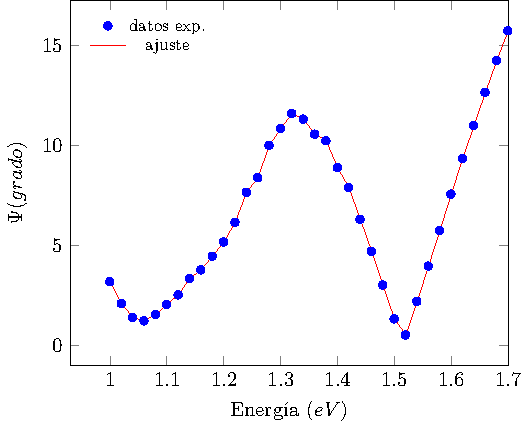
\includegraphics[scale=0.5]{figMet/figElips/grafPsi}
  		\label{Met:fig:PsiBS}
  	}
  	\subfigure[valores de $\Delta$]{
  		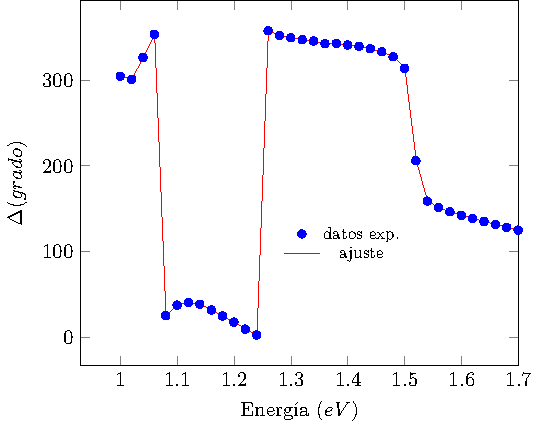
\includegraphics[scale=0.5]{figMet/figElips/grafTheta}
  		\label{Met:fig:DeltaBS}
  	}
  	\caption[Gr\'aficas de $\Psi$ y $\Delta$ del beamspliter a $70 \degree$.]{valores experimentales a $70\degree$  para $\Psi$ y $\Delta$ del beamsplitter en funci\'on de la energ\'ia del fot\'on con su ajuste.} 
  	\label{Met:fig:ElipBS}
  \end{figure}
}
\frame{
	\frametitle{Ajuste a 45 \degree}
	\begin{figure}[!hbt]
		\centering
		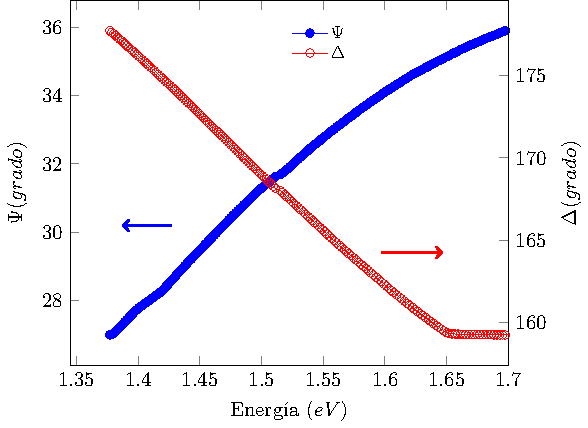
\includegraphics[scale=0.6]{figMet/figElips/grafPsidelta45.pdf}
		\caption[Gr\'aficas de $\Psi$ y $\Delta$ del beamspliter a $70 \degree$.]{valores calculados a $45\degree$  para $\Psi$ y $\Delta$ del beamsplitter.}
		\label{Met:fig:ElipBS45}
	\end{figure}
}
\endinput
	\subsection{mediciones}
\frame{
	\frametitle{Mediciones de hist\'eresis}
	\begin{itemize}
		\item Medidas con un diodo l\'aser con $\lambda= ~660~nm.$
	\end{itemize}
	\begin{figure}[!hbt]
		\centering
		\subfigure[Rotaci\'on Kerr]{
			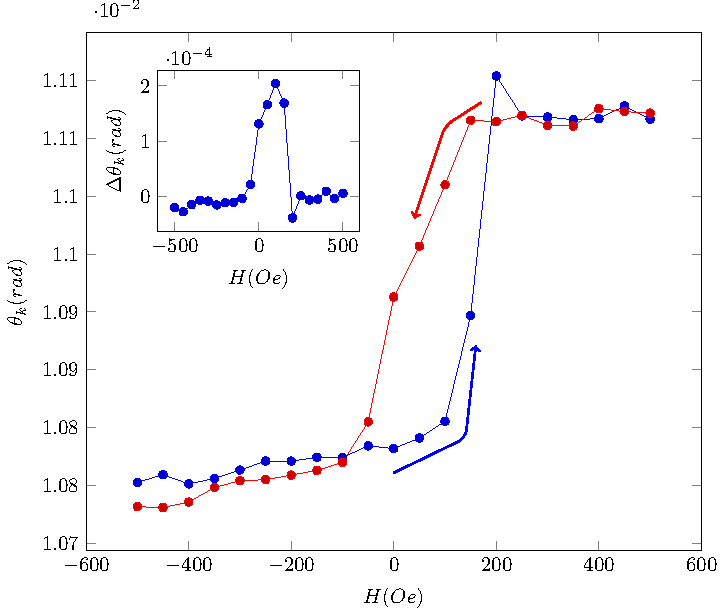
\includegraphics[scale=0.4]{resexp/his/HisTheta.pdf}
			\label{Exp:fig:theta}
		}
		\subfigure[Elipticidad Kerr]{
			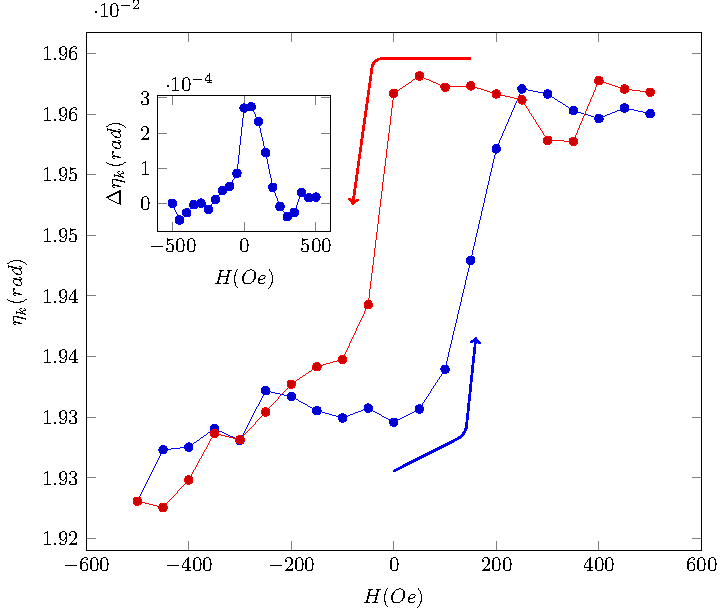
\includegraphics[scale=0.4]{resexp/his/HisEpsilon.pdf}
			\label{Exp:fig:elip}
		}
		\caption[Hit\'eresis de $\theta_k$ y $\eta_k$ en CoFeB]{Medici\'on de rotaci\'on (\ref{Exp:fig:theta}) y elipticidad (\ref{Exp:fig:elip}) Kerr enuna muestra de CoFeB. Dentro de cada figura se muestra en cambio de la se\~nal medida con cada direcci\'on de campo magn\'etico.}
		\label{Exp:fig:Kerrhis}
		
	\end{figure}
}
\frame{
\frametitle{Mediciones de espectro}
\begin{figure}[!hbt]
	\centering
	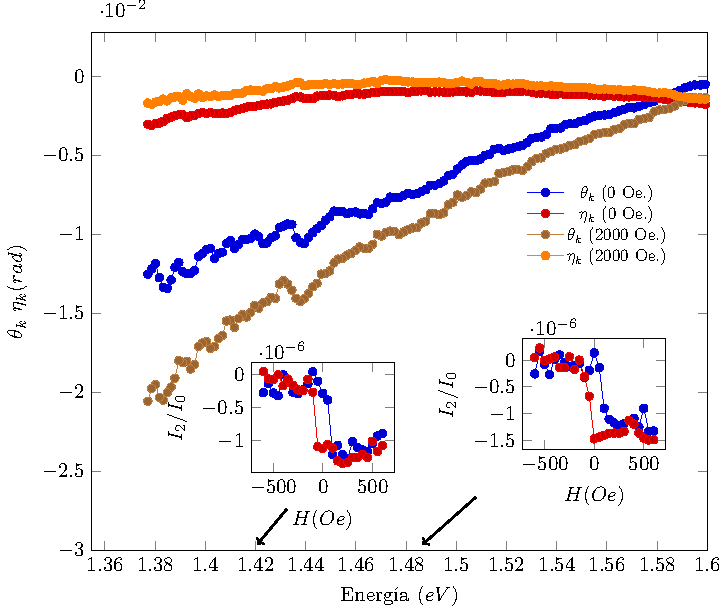
\includegraphics[scale=0.6]{resexp/esp/espectro0.pdf}
	\caption[Espectro de efecto Kerr magneto-\'optico]{Espectros del \'angulo y elipticidad Kerr en funci\'on de la energ\'ia del fot\'on en donde se induce un campo de $2000 Oe$. }
	\label{Exp:fig:espectroK}
\end{figure}
}
	\section{conclusiones}
\frame{
	\frametitle{Conclusiones}
	\begin{itemize}
		\item Se comenz\'o con el estudio de materiales bidimensionales llamados metales de dicalcogenuros de transición basados en  Platino y  Vanadio y utilizando el Azufre y Selenio como calc\'ogenos. 
		\item Al momento de estudiar estos materiales sin defectos, se observ\'o en el PtSe\textsubscript{2} y PtS\textsubscript{2} que no existe una magnetizaci\'on neta a pesar de que se observa un efecto spin-\'orbita considerable asociado principalmente al \'atomo  Platino. En el caso contrario,  para VSe\textsubscript{2} y  VS\textsubscript{2} si existe una magnetizaci\'on distinta de cero. Observando el comportamiento de la magnetizaci\'on en estos materiales se pudo notar que el cambio de Selenio o Azufre no afecta considerablemente a las propiedades magn\'eticas y por lo tanto  el cambio recae en el metal de transici\'on (Pt y V).
		
	\end{itemize}
}
\frame{
	\begin{itemize}
		\item se estudi\'o el efecto de introducir una vacancia del metal de transici\'on y se observ\'o que en el caso de los materiales con Platino, aparece una magnetizaci\'on que ronda en el valor de $2.5 \mu_{B}/celda$
		\item Para  el caso de los materiales con vanadio se  pudo observar que la magnetizaci\'on se reduce considerablemente a pesar de que la deformaci\'on del sistema es muy peque\~na.
		\item se pudo investigar el efecto que tiene una deformaci\'on mec\'anica isotr\'opica y anisotr\'opica en VSe\textsubscript{2} y VS\textsubscript{2} sin defectos; as\'i como en  PtSe\textsubscript{2} y PtS\textsubscript{2} con una vacancia de Platino.
	\end{itemize}
}
\frame{
		\frametitle{Conclusiones}
	\begin{itemize}
		\item Se logr\'o desarrollar un sistema de espectroscopia de Efecto Kerr magneto-\'optico partiendo de un montaje ya dise\~nado anteriormente y se desarroll\'o la instrumentaci\'on virtual para su control. 
		\item  fue necesario medir elipsometr\'ia a 70 \degree a dicho beamsplitter y   se escribi\'o un c\'odigo en Python para poder adquirir la rotaci\'on ($\theta_k$) y la elipticidad ($\eta_k$)  Kerr tanto de las mediciones de hist\'eresis como del espectro a incidencia casi normal con el beamsplitter a 45 \degree.
		\item se midi\'o la hist\'eresis y espectro Kerr de una muestra de CoFeB depositada sobre Sio\textsubscript{2}
	\end{itemize}
} 
	\section{Bibliograf\'ia}
	\frame{
		\frametitle{Bibliograf\'ia}
		
		\printbibliography

	}
   \section*{}
   \frame{
   	\Large{\centering \bf\textcolor{blue}{ ¡Gracias por su atenci\'on ! }}\\[ 5 mm]
   }
\end{document}